\section{Evolution of vertex degree for different arrival times} \label{app:evolution}

\begin{figure}[ht]
\centering
\begin{subfigure}{.5\textwidth}
  \centering
  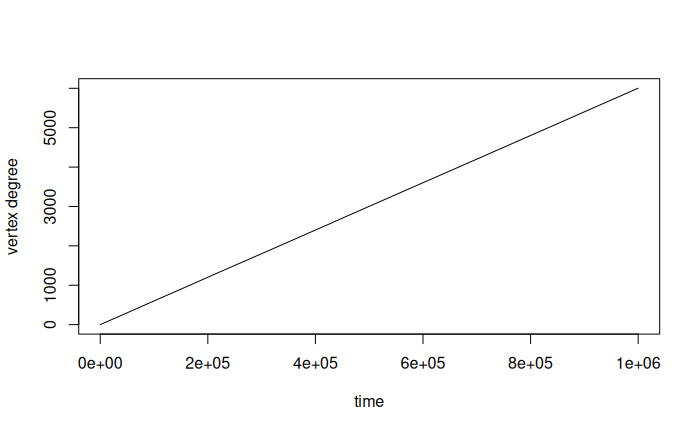
\includegraphics[width=\linewidth]{figures/scaling_NG/sc_ng_0.png}
\end{subfigure}%
\begin{subfigure}{.5\textwidth}
  \centering
  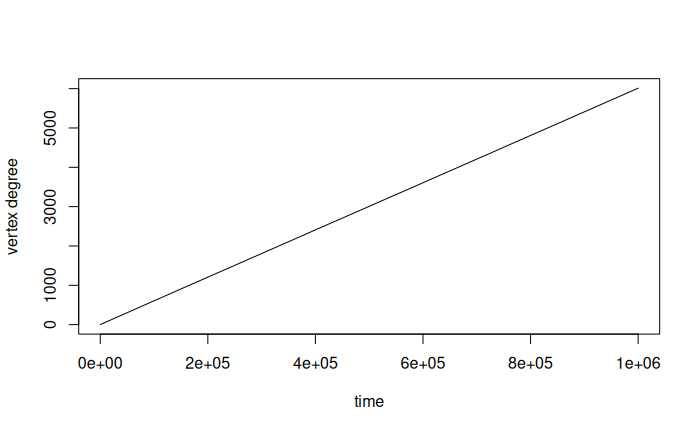
\includegraphics[width=\linewidth]{figures/scaling_NG/sc_ng_1.png}
\end{subfigure}
\begin{subfigure}{.5\textwidth}
  \centering
  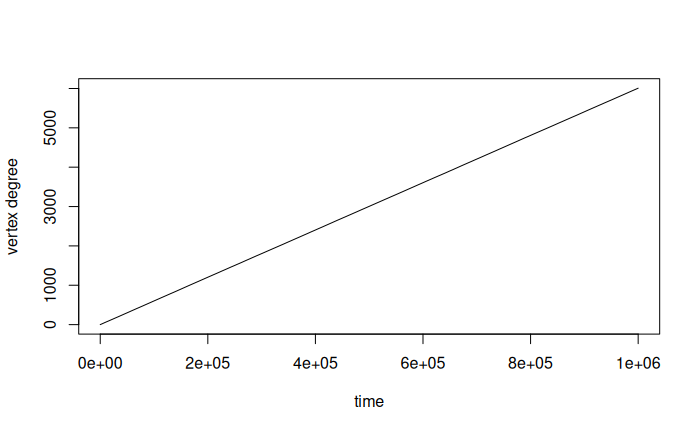
\includegraphics[width=\linewidth]{figures/scaling_NG/sc_ng_2.png}
\end{subfigure}
\caption{Vertex degree at every time step of a \textit{No Growth + Preferential Attachment} model for vertices with arrival times (from left to right, top to bottom): 1, 10, 100.}
\label{fig:scaling_NG}
\end{figure}

\begin{figure}[ht]
\centering
\begin{subfigure}{.5\textwidth}
  \centering
  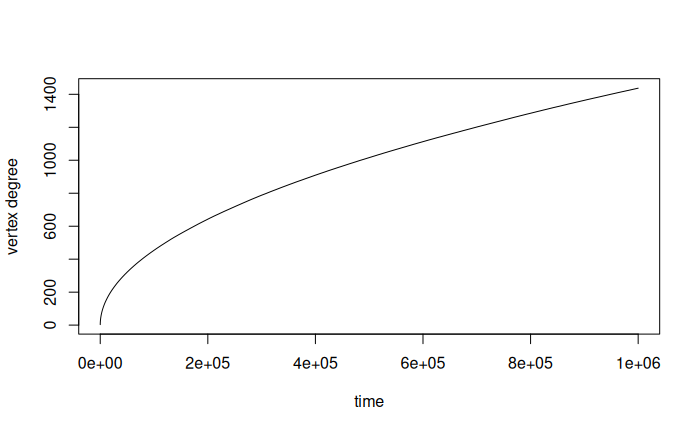
\includegraphics[width=\linewidth]{figures/scaling_BA/sc_ba_0.png}
\end{subfigure}%
\begin{subfigure}{.5\textwidth}
  \centering
  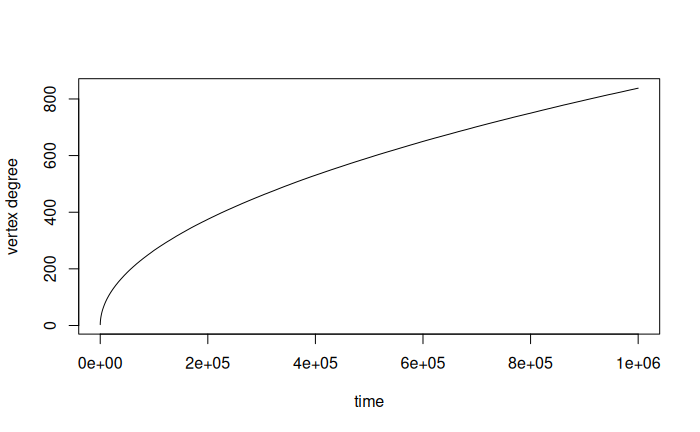
\includegraphics[width=\linewidth]{figures/scaling_BA/sc_ba_1.png}
\end{subfigure}
\begin{subfigure}{.5\textwidth}
  \centering
  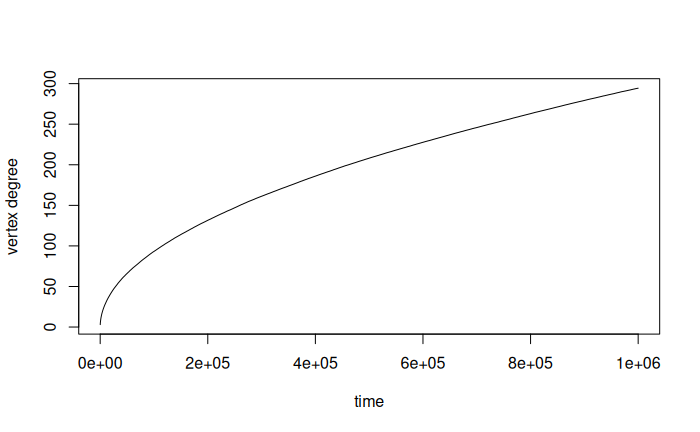
\includegraphics[width=\linewidth]{figures/scaling_BA/sc_ba_2.png}
\end{subfigure}%
\begin{subfigure}{.5\textwidth}
  \centering
  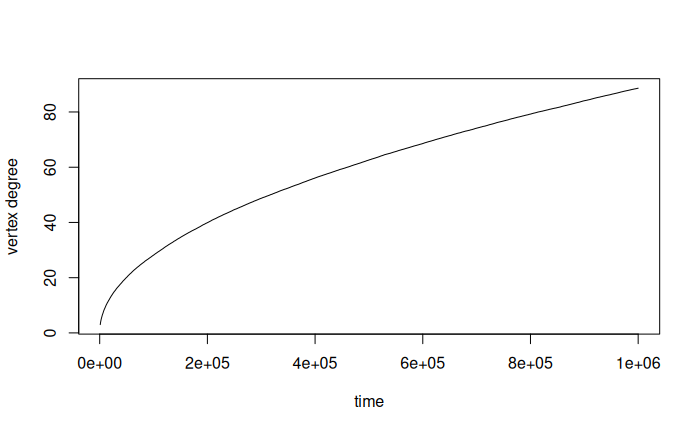
\includegraphics[width=\linewidth]{figures/scaling_BA/sc_ba_3.png}
\end{subfigure}
\begin{subfigure}{.5\textwidth}
  \centering
  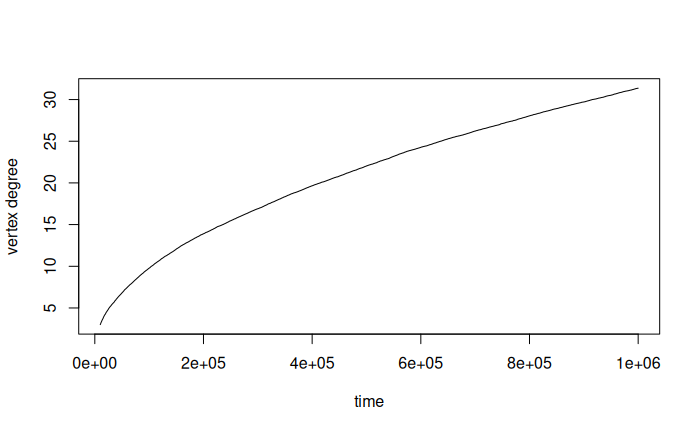
\includegraphics[width=\linewidth]{figures/scaling_BA/sc_ba_4.png}
\end{subfigure}%
\begin{subfigure}{.5\textwidth}
  \centering
  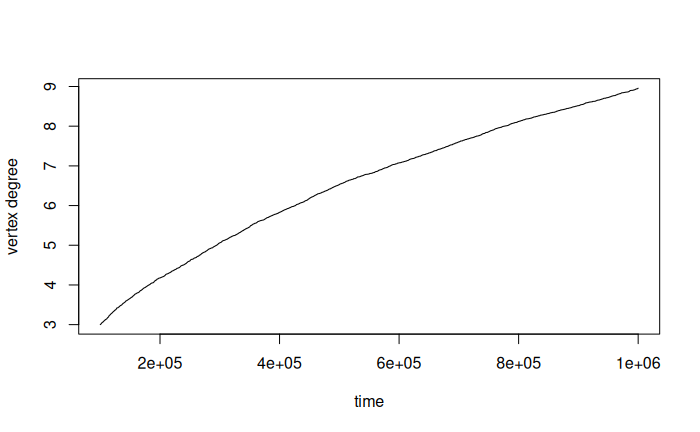
\includegraphics[width=\linewidth]{figures/scaling_BA/sc_ba_5.png}
\end{subfigure}
\caption{Vertex degree at every time step of a \textit{Barabási-Albert} model for vertices with arrival times (from left to right, top to bottom): 1, 10, 100, 1000, 10000, 100000.}
\label{fig:scaling_BA}
\end{figure}

\begin{figure}[ht]
\centering
\begin{subfigure}{.5\textwidth}
  \centering
  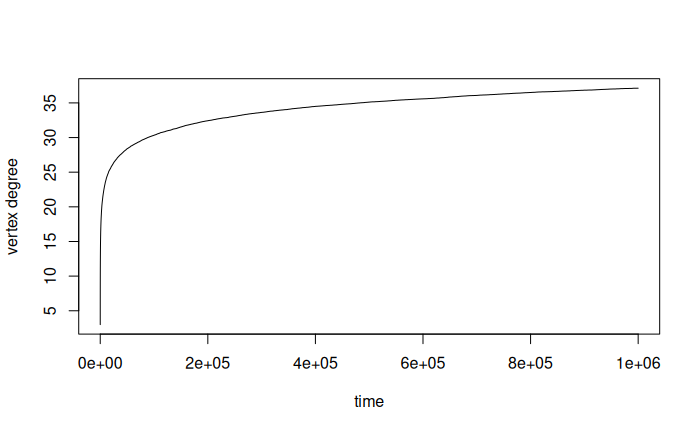
\includegraphics[width=\linewidth]{figures/scaling_RA/sc_ra_0.png}
\end{subfigure}%
\begin{subfigure}{.5\textwidth}
  \centering
  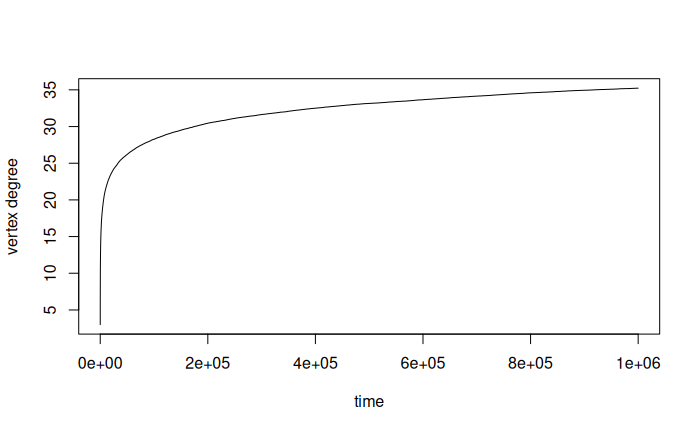
\includegraphics[width=\linewidth]{figures/scaling_RA/sc_ra_1.png}
\end{subfigure}
\begin{subfigure}{.5\textwidth}
  \centering
  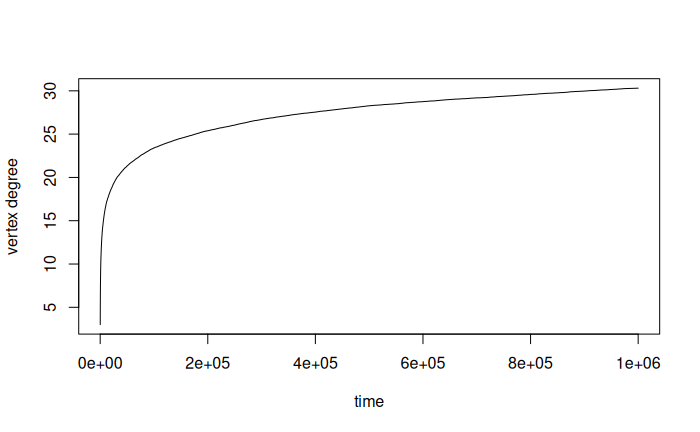
\includegraphics[width=\linewidth]{figures/scaling_RA/sc_ra_2.png}
\end{subfigure}%
\begin{subfigure}{.5\textwidth}
  \centering
  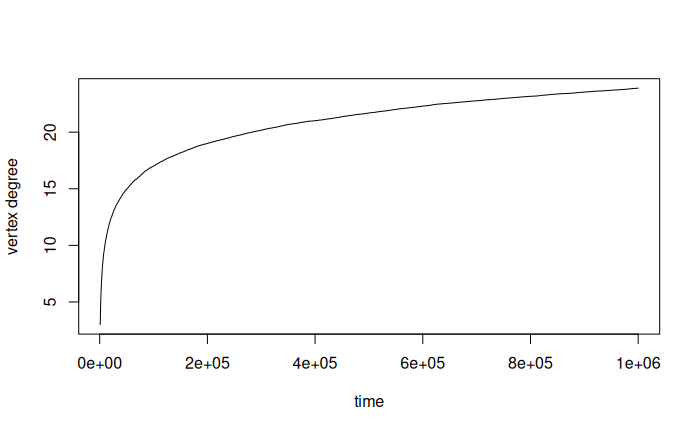
\includegraphics[width=\linewidth]{figures/scaling_RA/sc_ra_3.png}
\end{subfigure}
\begin{subfigure}{.5\textwidth}
  \centering
  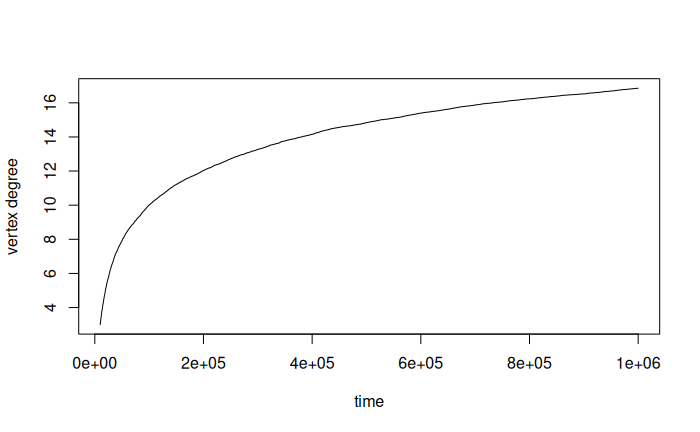
\includegraphics[width=\linewidth]{figures/scaling_RA/sc_ra_4.png}
\end{subfigure}%
\begin{subfigure}{.5\textwidth}
  \centering
  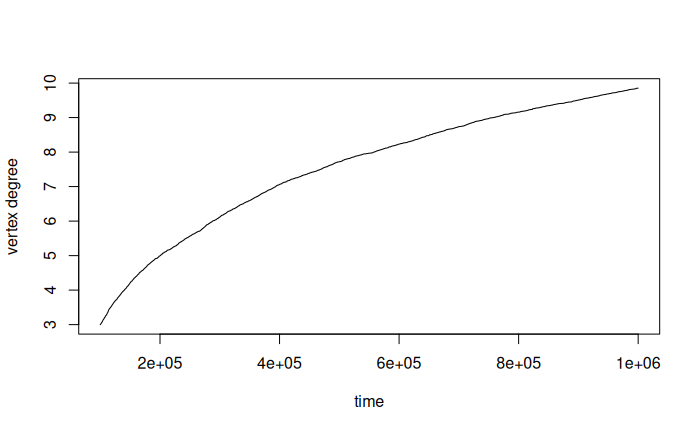
\includegraphics[width=\linewidth]{figures/scaling_RA/sc_ra_5.png}
\end{subfigure}
\caption{Vertex degree at every time step of a \textit{Growth + Random Attachment} model for vertices with arrival times (from left to right, top to bottom): 1, 10, 100, 1000, 10000, 100000.}
\label{fig:scaling_RA}
\end{figure}


\newpage
\section{Fit of the curves modeling the scaling of vertex degree over time} \label{app:sca_fit}

\begin{figure}[ht]
\centering
\begin{subfigure}{.5\textwidth}
  \centering
  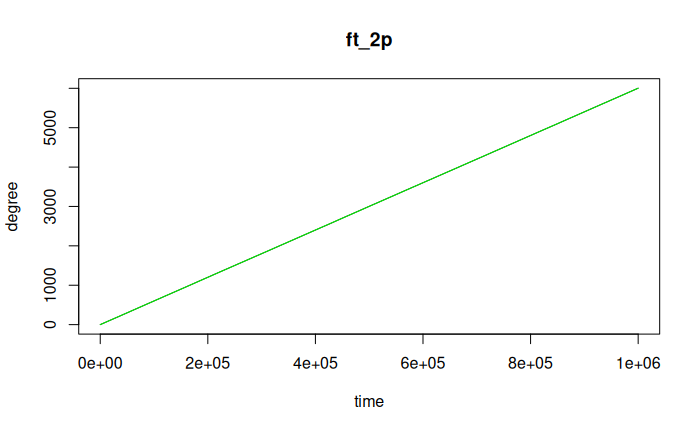
\includegraphics[width=\linewidth]{figures/scaling_fits/fit_ng_0.png}
\end{subfigure}%
\begin{subfigure}{.5\textwidth}
  \centering
  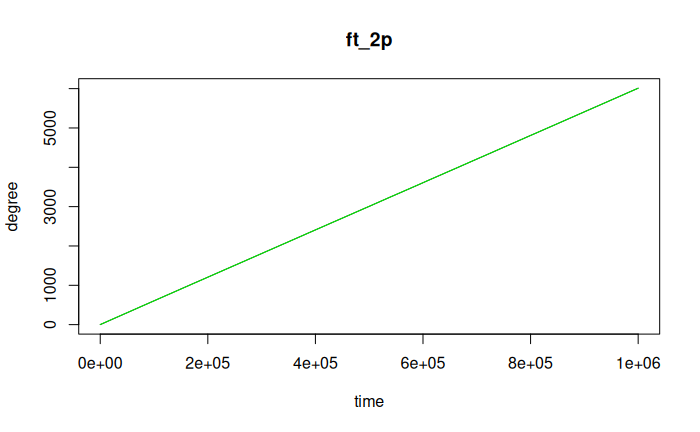
\includegraphics[width=\linewidth]{figures/scaling_fits/fit_ng_1.png}
\end{subfigure}
\begin{subfigure}{.5\textwidth}
  \centering
  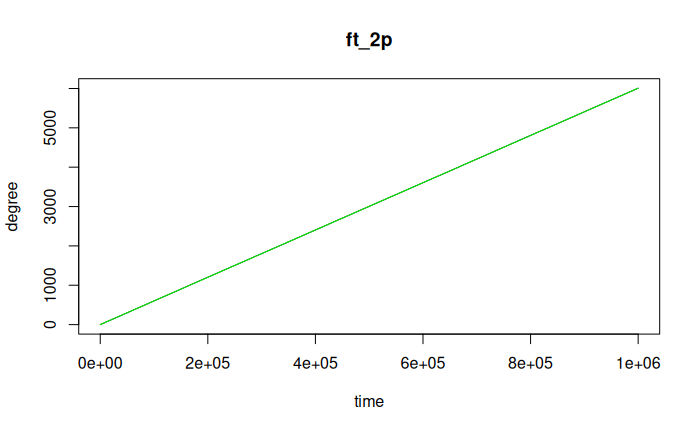
\includegraphics[width=\linewidth]{figures/scaling_fits/fit_ng_2.png}
\end{subfigure}
\caption{Fitted curve (green) on top of the curve showing vertex degree evolution (black) for the \textit{No Growth + Preferential Attachment} model.}
\label{fig:fit_NG}
\end{figure}

\begin{figure}[ht]
\centering
\begin{subfigure}{.5\textwidth}
  \centering
  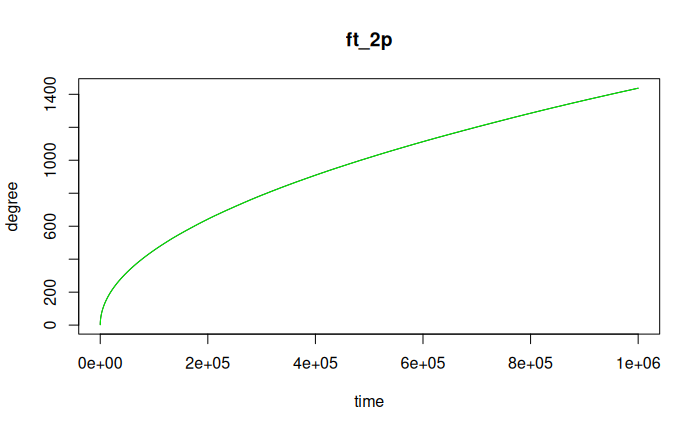
\includegraphics[width=\linewidth]{figures/scaling_fits/fit_ba_0.png}
\end{subfigure}%
\begin{subfigure}{.5\textwidth}
  \centering
  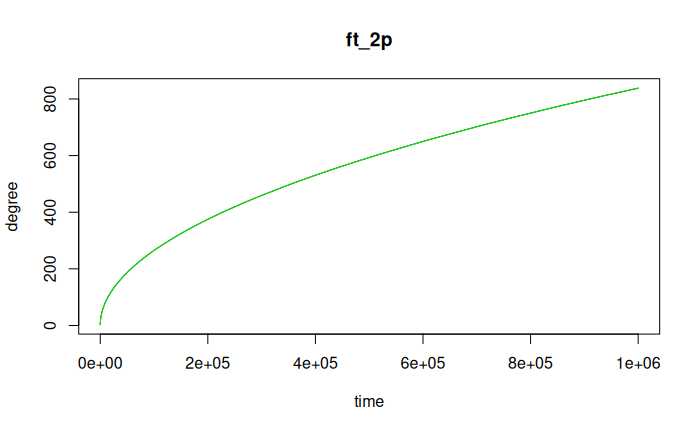
\includegraphics[width=\linewidth]{figures/scaling_fits/fit_ba_1.png}
\end{subfigure}
\begin{subfigure}{.5\textwidth}
  \centering
  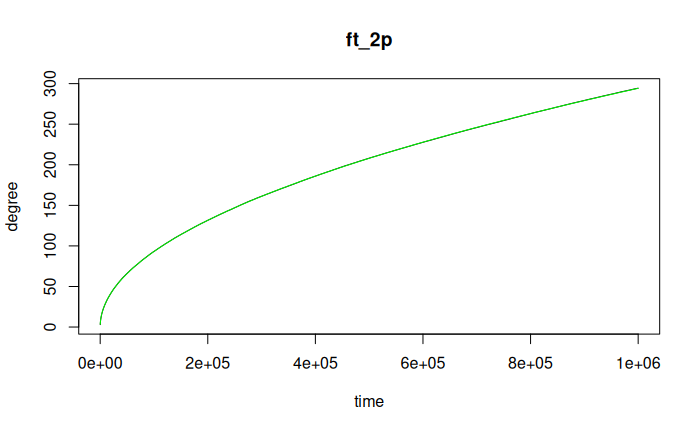
\includegraphics[width=\linewidth]{figures/scaling_fits/fit_ba_2.png}
\end{subfigure}%
\begin{subfigure}{.5\textwidth}
  \centering
  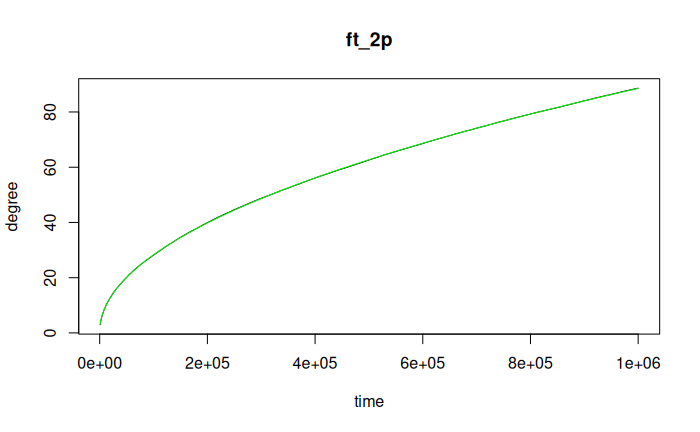
\includegraphics[width=\linewidth]{figures/scaling_fits/fit_ba_3.png}
\end{subfigure}
\begin{subfigure}{.5\textwidth}
  \centering
  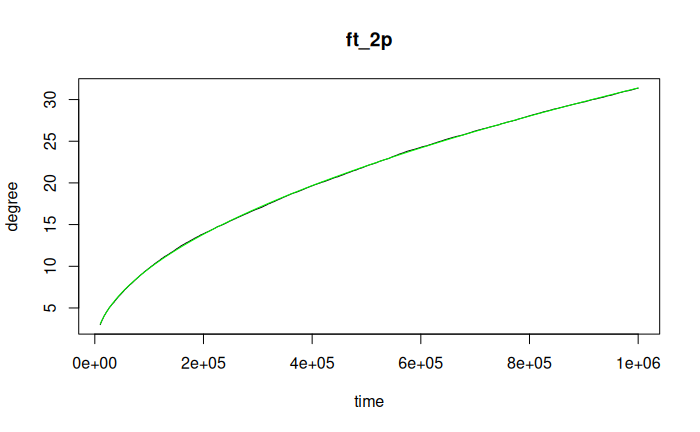
\includegraphics[width=\linewidth]{figures/scaling_fits/fit_ba_4.png}
\end{subfigure}%
\begin{subfigure}{.5\textwidth}
  \centering
  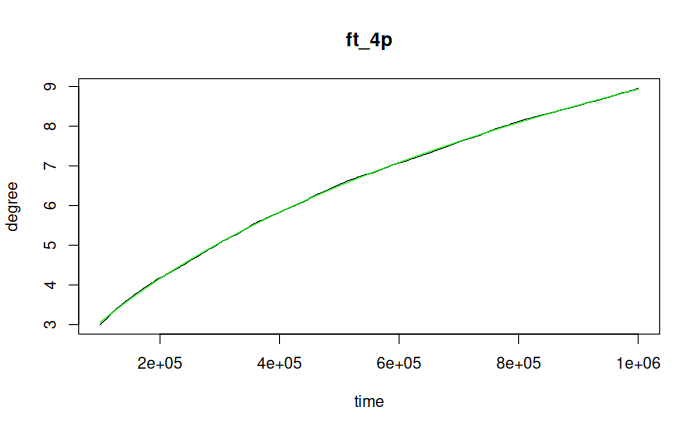
\includegraphics[width=\linewidth]{figures/scaling_fits/fit_ba_5.png}
\end{subfigure}
\caption{Fitted curve (green) on top of the curve showing vertex degree evolution (black) for the \textit{Barabási-Albert} model.}
\label{fig:fit_BA}
\end{figure}

\begin{figure}[ht]
\centering
\begin{subfigure}{.5\textwidth}
  \centering
  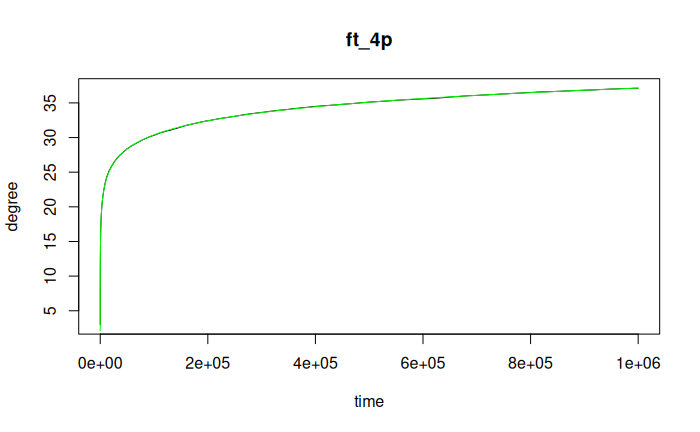
\includegraphics[width=\linewidth]{figures/scaling_fits/fit_ra_0.png}
\end{subfigure}%
\begin{subfigure}{.5\textwidth}
  \centering
  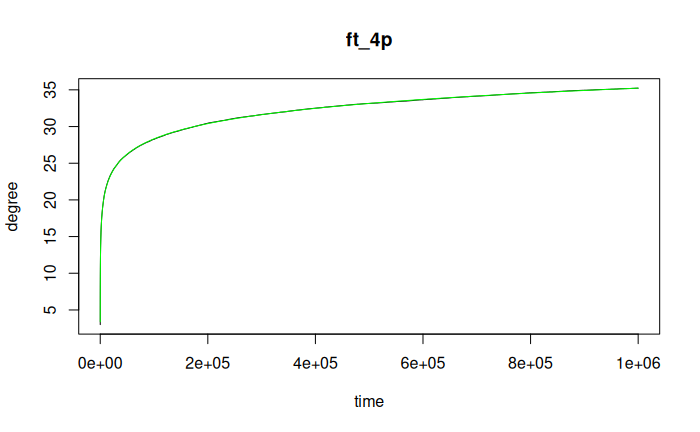
\includegraphics[width=\linewidth]{figures/scaling_fits/fit_ra_1.png}
\end{subfigure}
\begin{subfigure}{.5\textwidth}
  \centering
  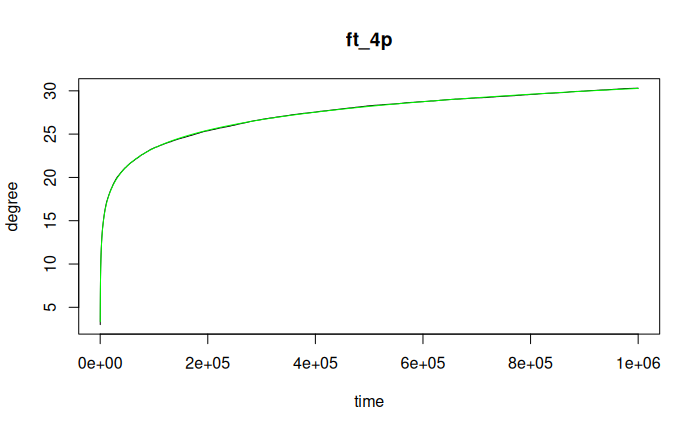
\includegraphics[width=\linewidth]{figures/scaling_fits/fit_ra_2.png}
\end{subfigure}%
\begin{subfigure}{.5\textwidth}
  \centering
  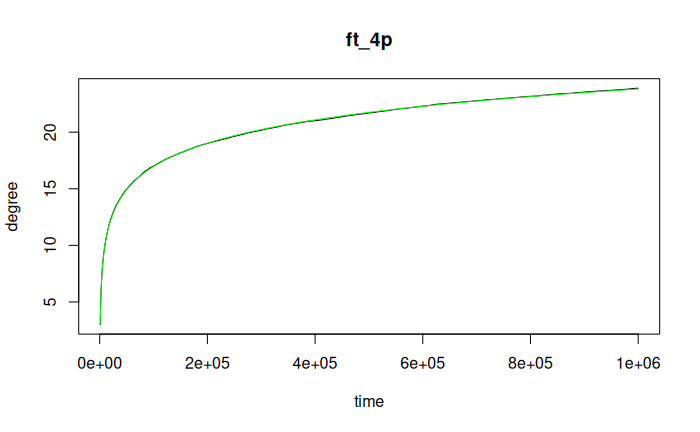
\includegraphics[width=\linewidth]{figures/scaling_fits/fit_ra_3.png}
\end{subfigure}
\begin{subfigure}{.5\textwidth}
  \centering
  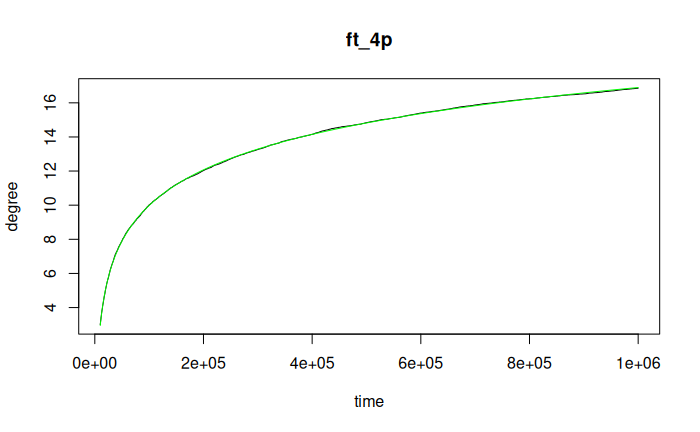
\includegraphics[width=\linewidth]{figures/scaling_fits/fit_ra_4.png}
\end{subfigure}%
\begin{subfigure}{.5\textwidth}
  \centering
  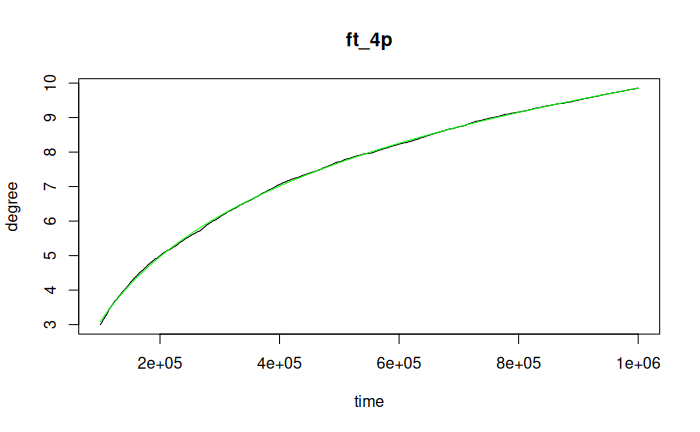
\includegraphics[width=\linewidth]{figures/scaling_fits/fit_ra_5.png}
\end{subfigure}
\caption{Fitted curve (green) on top of the curve showing vertex degree evolution (black) for the \textit{Growth + Random Attachment} model.}
\label{fig:fit_RA}
\end{figure}


\newpage
\section{Curves of the fitted degree distributions over the data} \label{app:degseq}

\begin{figure}[ht]
\centering
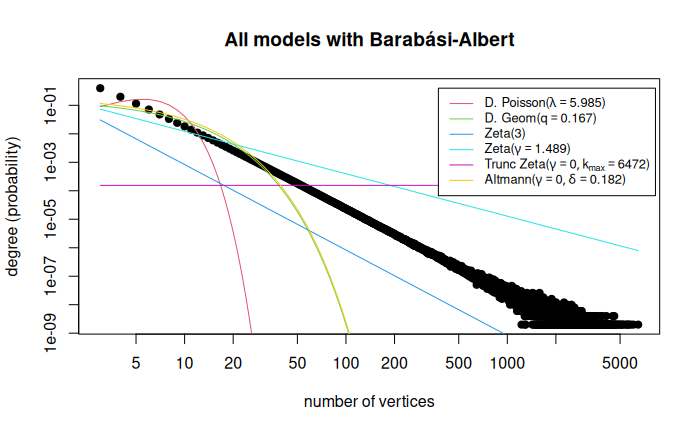
\includegraphics[width=0.8\linewidth]{figures/degseq_fits/BA_degseq.png}
\caption{Plot of the degree distribution of the \textit{Barabási-Albert} model in a log-log scale, with the curves of the fitted distributions overlaid.}
\label{fig:degseq_BA}
\end{figure}
% TODO: fix image, artificial lowering

\begin{figure}[ht]
\centering
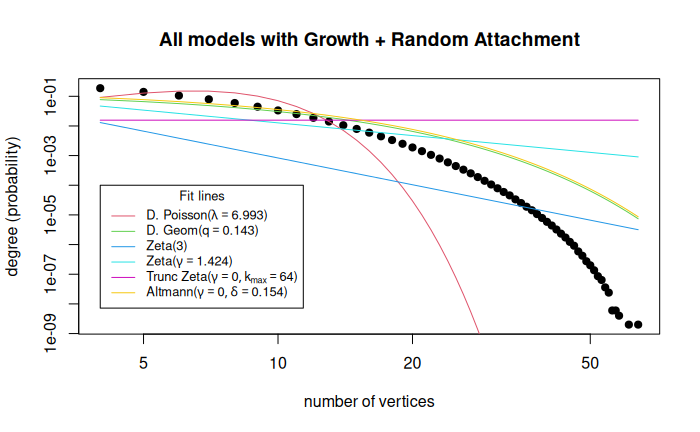
\includegraphics[width=0.8\linewidth]{figures/degseq_fits/RA_degseq.png}
\caption{Plot of the degree distribution of the \textit{Growth + Random Attachment} model in a log-log scale, with the curves of the fitted distributions overlaid.}
\label{fig:degseq_RA}
\end{figure}

\begin{figure}[ht]
\centering
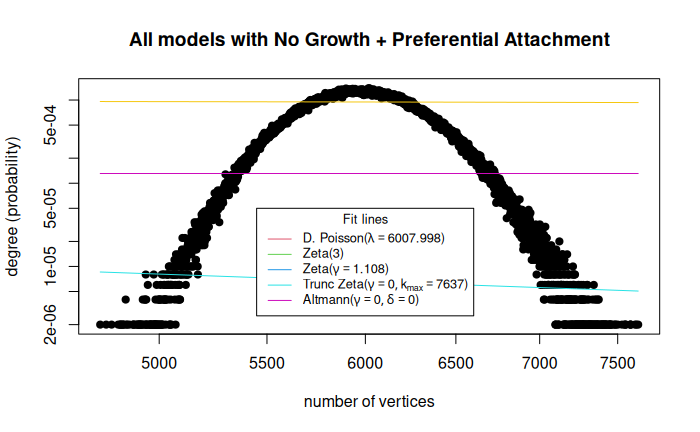
\includegraphics[width=0.8\linewidth]{figures/degseq_fits/NG_degseq.png}
\caption{Plot of the degree distribution of the \textit{No Growth + Preferencial Attachment} model in a log-log scale, with the curves of the fitted distributions overlaid.}
\label{fig:degseq_NG}
\end{figure}